\section{Kết quả triển khai sản phẩm}

Dựa trên quá trình triển khai và vận hành thực tế hệ thống, phần này tổng kết các kết quả đạt được so với các thiết kế ban đầu, đánh giá mức độ hoàn thành mục tiêu và đề xuất hướng phát triển cho tương lai.

\subsection{Kết quả đạt được so với thiết kế}

Quá trình hiện thực hóa nguyên mẫu (prototype) đã bám sát các thiết kế từ \autoref{chap:hien_thuc}, cụ thể:

\begin{itemize}
    \item \textbf{Về phần cứng (Hardware):} Đã chế tạo thành công bo mạch chính (Baseboard) với cấu trúc PCB 6 lớp, đảm bảo tính toàn vẹn tín hiệu cho các giao tiếp tốc độ cao. Hệ thống Dual-MCU (Master-Slave) sử dụng hai vi điều khiển ESP32-S3 vận hành đúng theo thiết kế. Các khe cắm mở rộng (WAN, LAN1, LAN2) tương thích hoàn toàn với các Module Adapter, cho phép tháo lắp và thay đổi linh hoạt các chuẩn kết nối vật lý.
    \item \textbf{Về phần mềm (Firmware):} Hệ thống Firmware dựa trên RTOS đã được triển khai hiệu quả trên cả hai MCU. Cơ chế giao tiếp nội bộ Inter-MCU thông qua giao thức Quad SPI với GPIO Handshake Event-driven (thay thế Polling của phiên bản nguyên mẫu) đạt tốc độ truyền tải dữ liệu đúng như kỳ vọng, đảm bảo không có độ trễ đáng kể trong việc điều phối dữ liệu giữa các lớp mạng.
    \item \textbf{Khả năng kết nối:} Sản phẩm đã thực hiện kết nối thành công với hạ tầng đám mây thông qua Wi-Fi, Ethernet (W5500) và LTE. Cơ chế Internet Monitor hoạt động đúng, tự động thay thế giao diện khi phát hiện mất kết nối. Đồng thời, hệ thống đã đọc và xử lý chính xác dữ liệu từ các cảm biến/thiết bị đầu cuối sử dụng giao thức LoRa, Zigbee, BLE Native/GATT, CAN và RS-485 thông qua các module chuyển đổi tương ứng. Hệ thống tự động phát hiện module (auto module detection) từ NVS khi khởi động.
\end{itemize}

\subsection{Kết quả kết nối thiết bị đầu cuối}

Để kiểm chứng khả năng tích hợp đa giao thức, hệ thống IoT Gateway được triển khai thử nghiệm thực tế cùng với nhiều thiết bị đầu cuối hoạt động đồng thời. Cụ thể, các thiết bị kết nối vào hệ thống bao gồm:

\begin{itemize}
    \item \textbf{BLE (Bluetooth Low Energy):} Các node cảm biến nhiệt độ--độ ẩm (DA2\_SENSOR) và thiết bị LED GATT (DA2\_LED\_GATT) giao tiếp trực tiếp qua BLE Native với LAN-MCU.
    \item \textbf{Zigbee:} Node cảm biến Zigbee (E180-ZG120B, EBYTE) kết nối qua LAN Adapter, dữ liệu được chuyển tiếp lên LAN-MCU qua UART.
    \item \textbf{LoRa P2P:} Node đầu cuối (Wio-E5-LE mini) truyền dữ liệu theo giao thức LoRa Point-to-Point, thu thập qua LAN Adapter.
    \item \textbf{MQTT Broker cục bộ:} Raspberry Pi đóng vai trò server MQTT (Mosquitto), nhận dữ liệu telemetry từ Gateway và cung cấp dashboard giám sát qua ThingsBoard.
\end{itemize}

\begin{figure}[H]
    \centering
    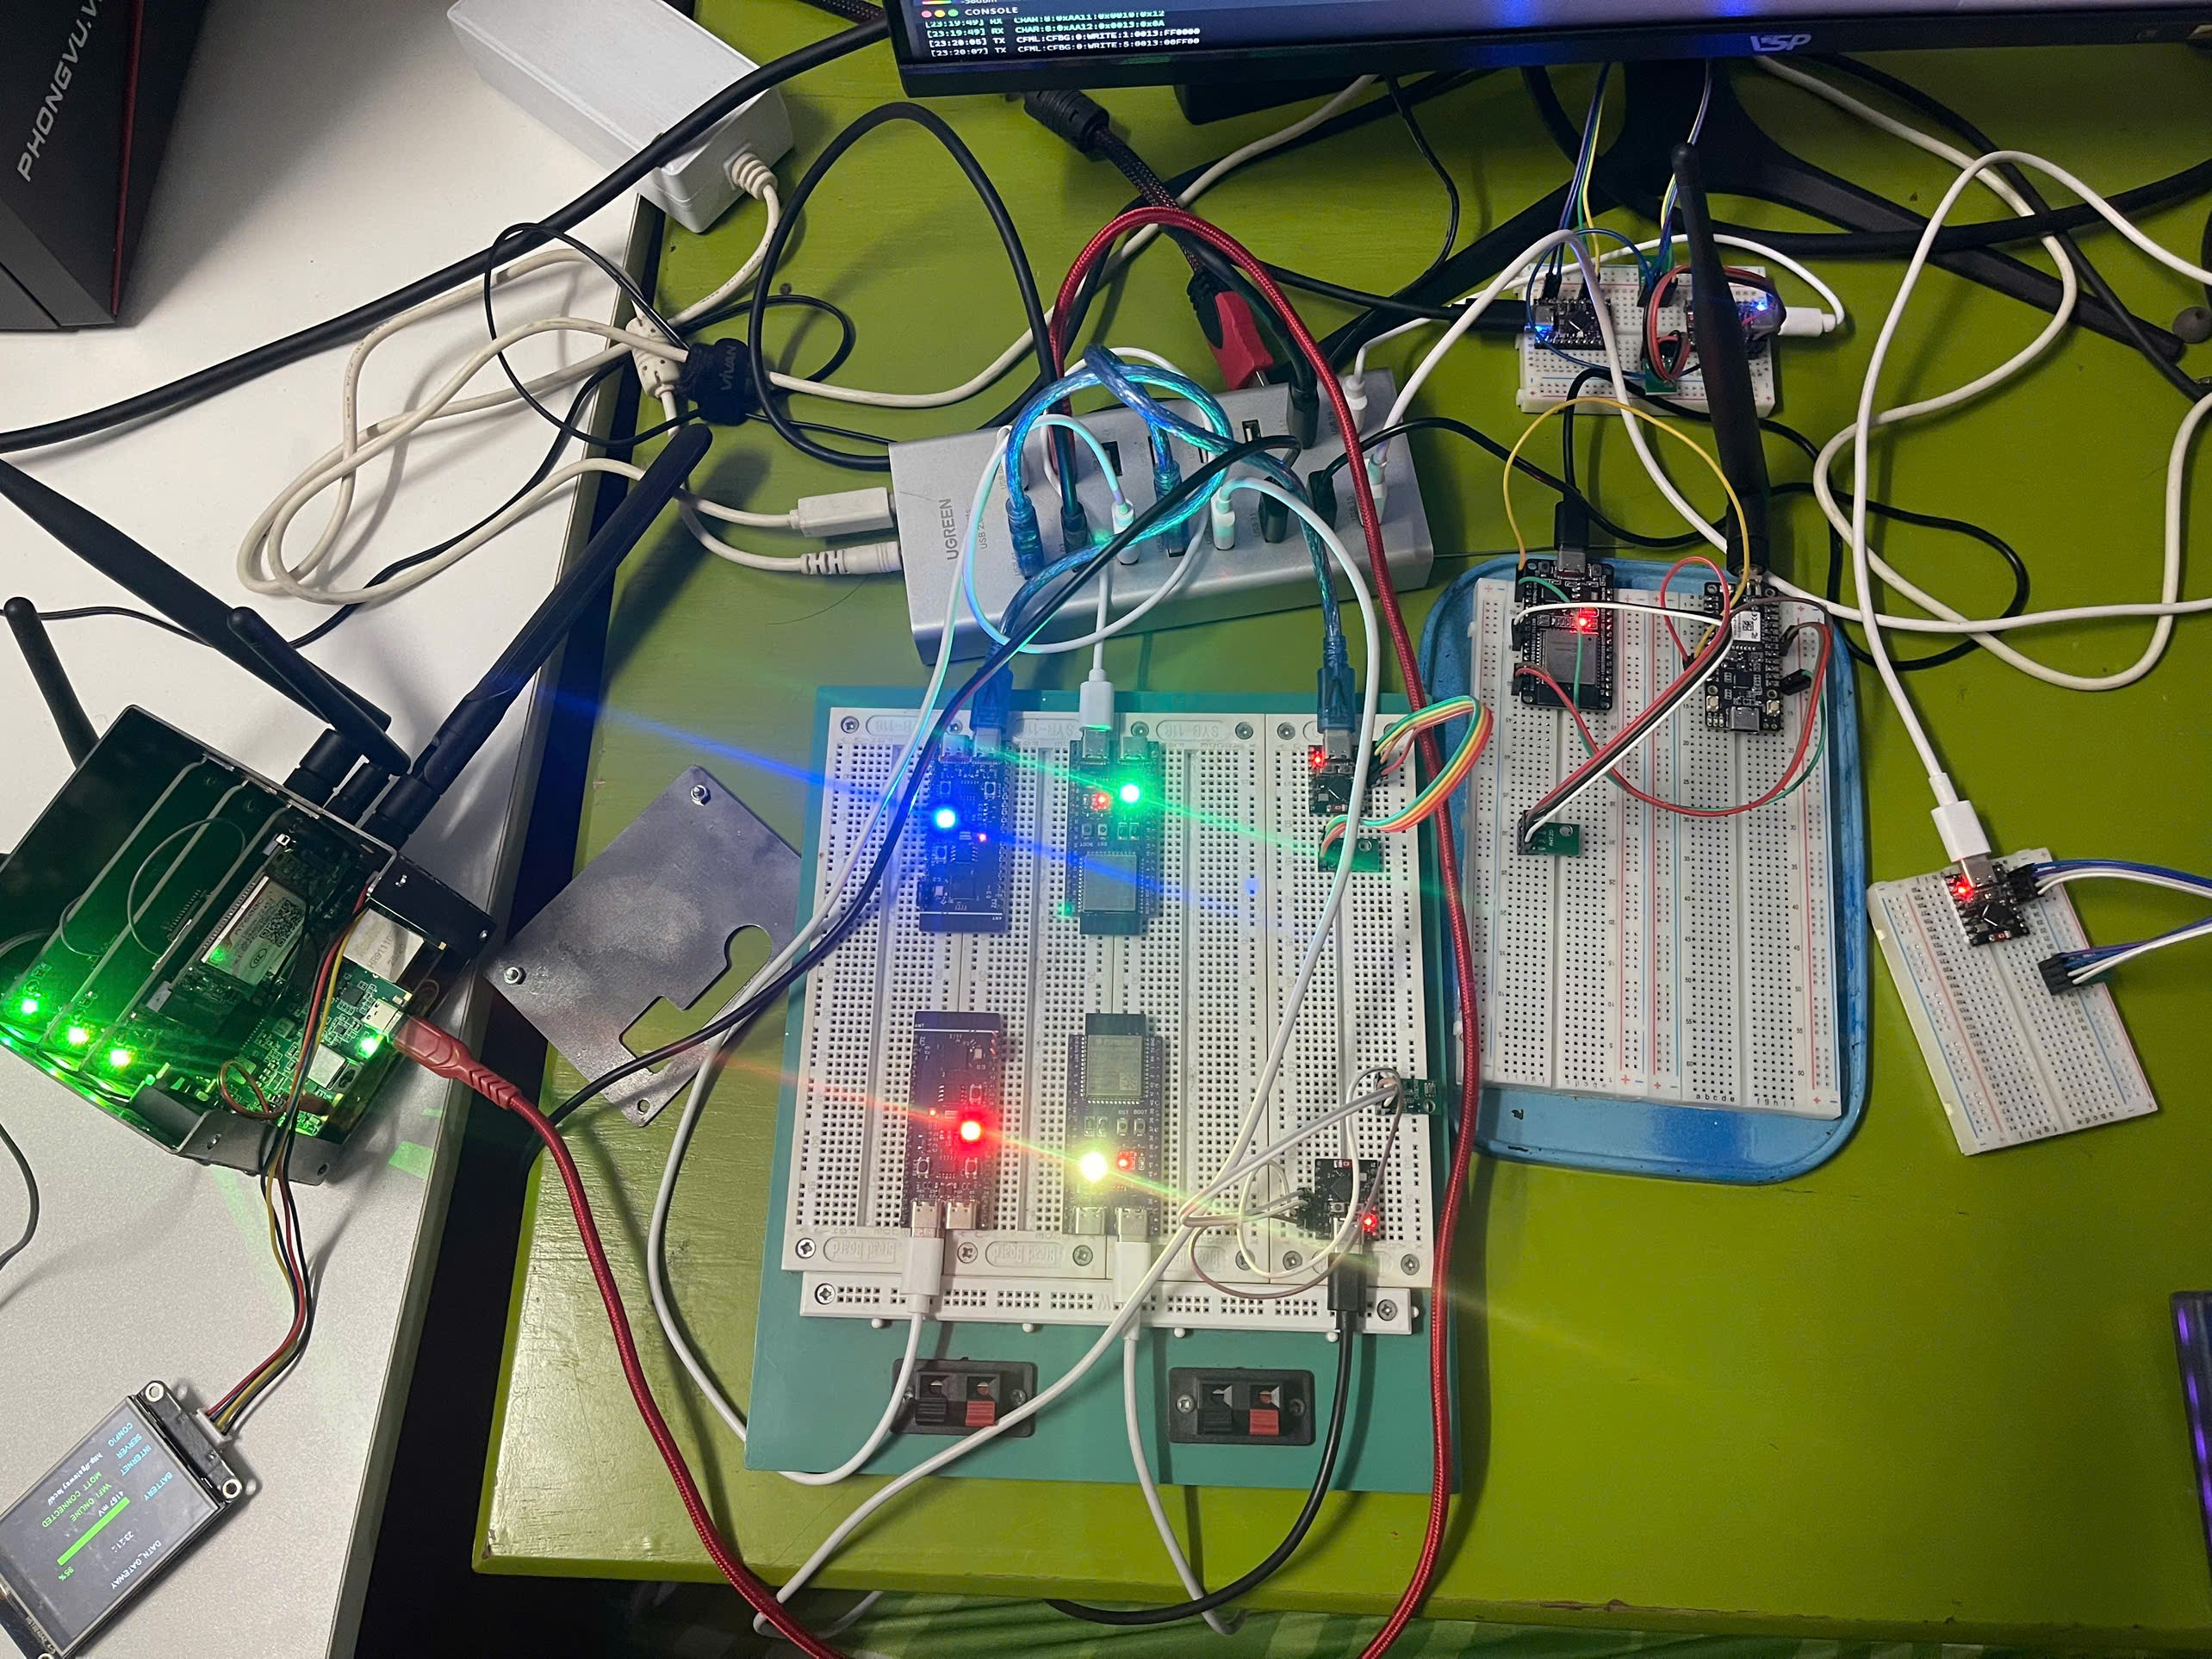
\includegraphics[width=0.9\textwidth]{figures/DATN/trien_khai_ket_noi.png}
    \caption{IoT Gateway kết nối đồng thời với các thiết bị đầu cuối BLE, Zigbee và LoRa P2P.}
    \label{fig:trien_khai_ket_noi}
\end{figure}

Kết quả cho thấy gateway nhận diện tự động tất cả module adapter đang cắm (dựa trên Device ID 4-bit từ IO Expander), khởi tải driver tương ứng từ NVS và thiết lập kênh truyền dữ liệu liên tục lên cloud mà không cần can thiệp thủ công vào firmware.

\subsection{Giao diện giám sát và quản lý thiết bị đầu cuối}

Trong quá trình thử nghiệm tích hợp, hệ thống gateway vận hành đồng thời với các thiết bị đầu cuối thuộc ba giao thức BLE, Zigbee và LoRa P2P. Dữ liệu telemetry từ tất cả thiết bị được tổng hợp tại Gateway, đóng gói theo định dạng JSON và đẩy liên tục lên MQTT Broker (Mosquitto trên Raspberry Pi), sau đó hiển thị trên dashboard ThingsBoard.

\begin{figure}[H]
    \centering
    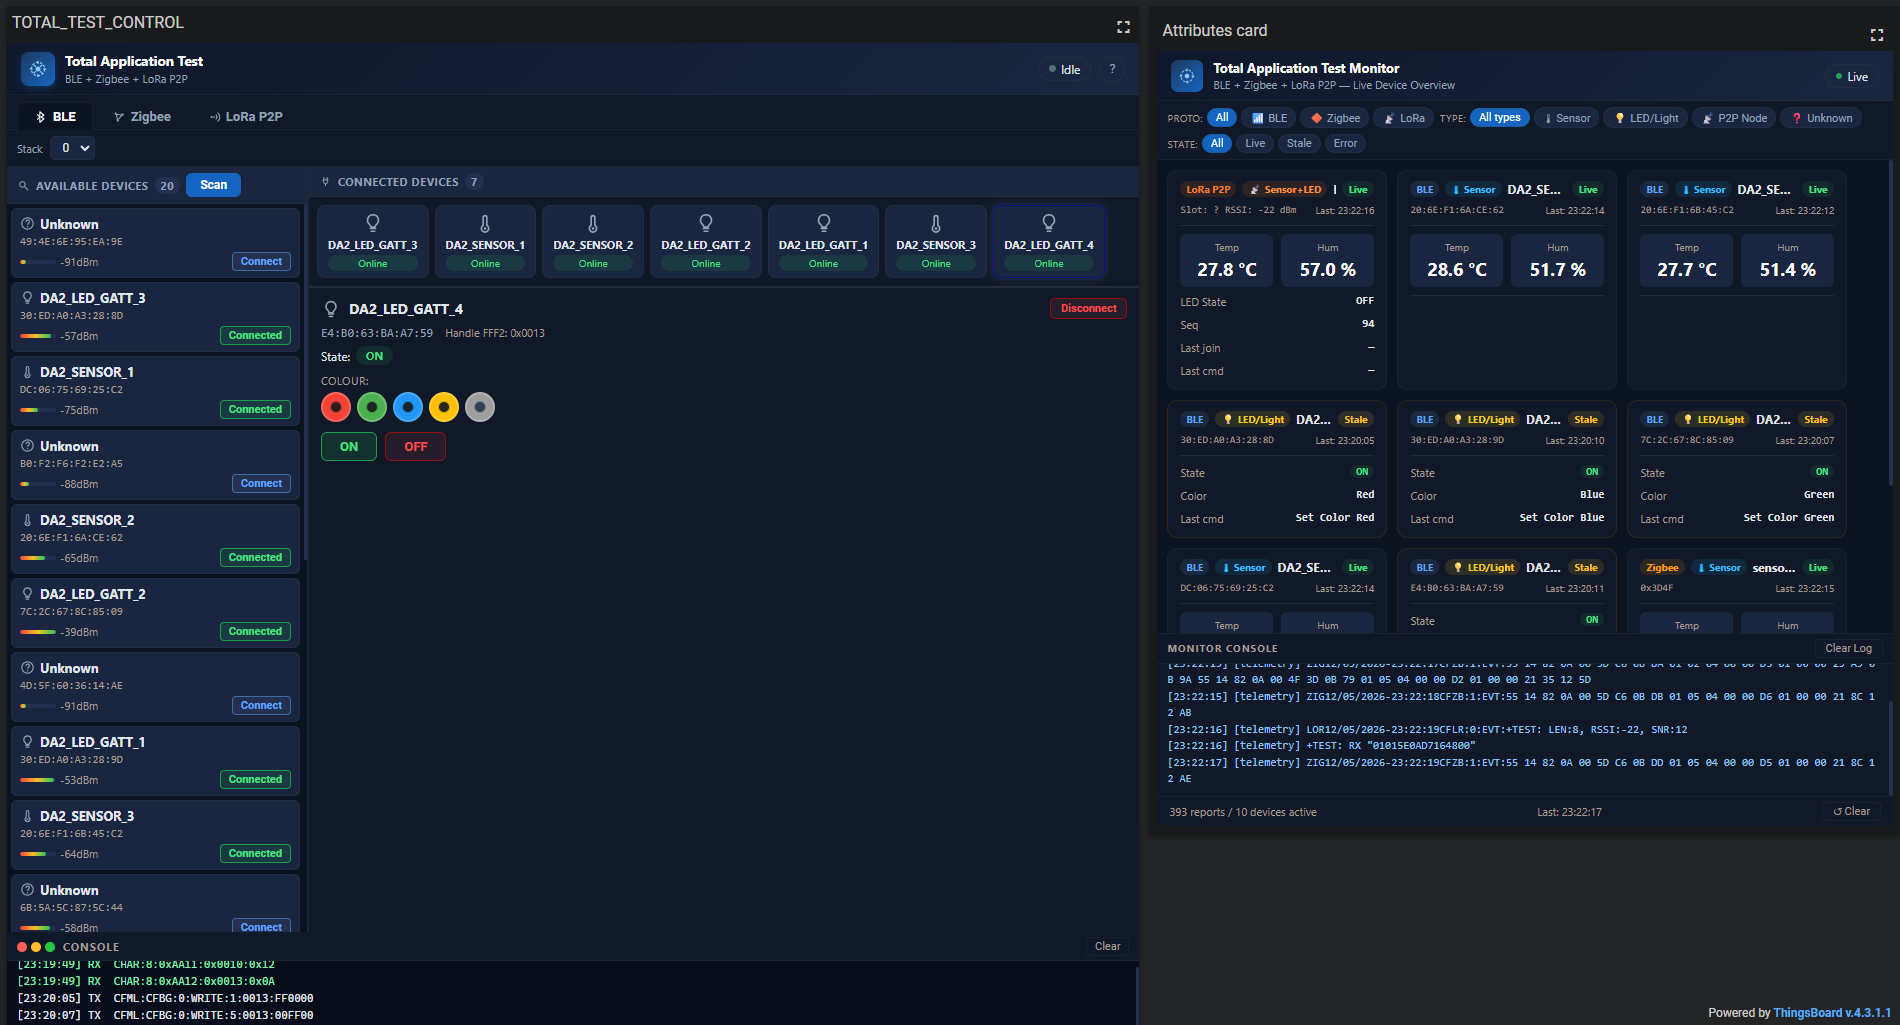
\includegraphics[width=\textwidth]{figures/giao_dien.png}
    \caption{Dashboard giám sát thiết bị.}
    \label{fig:monitor_dashboard}
\end{figure}

Giao diện giám sát cung cấp các chức năng cốt lõi:
\begin{itemize}
    \item \textbf{Quét và kết nối thiết bị:} Danh sách \textit{Available Devices} hiển thị 20 thiết bị BLE khả dụng trong vùng phủ sóng. Người dùng có thể nhấn \textit{Connect/Disconnect} để quản lý từng kết nối độc lập.
    \item \textbf{Giám sát trạng thái:} Panel \textit{Connected Devices} hiển thị trạng thái tất cả node đang kết nối (Online/Stale), cùng địa chỉ MAC, thời điểm cập nhật cuối và giá trị thuộc tính mới nhất (nhiệt độ 27.7--28.6$^\circ$C, độ ẩm 51--57\%).
    \item \textbf{Điều khiển thiết bị từ xa (Downlink):} Với node LED GATT, người dùng có thể chọn màu sắc (đỏ, xanh lá, xanh dương, vàng, trắng) và gửi lệnh ON/OFF trực tiếp từ dashboard. Lệnh được WAN-MCU nhận qua MQTT Subscribe, chuyển tiếp xuống LAN-MCU qua Quad SPI, sau đó LAN-MCU phát BLE GATT Write đến thiết bị.
    \item \textbf{Monitor Console:} Hiển thị log telemetry thời gian thực bao gồm dữ liệu BLE EVT, ZigBee report và LoRa Frame với timestamp, RSSI và SNR. Dòng log \texttt{[Telemetry] ZIG12/...EVT:55} và \texttt{CFLR0:EVT+TEST} xác nhận gateway xử lý đồng thời đa giao thức mà không có xung đột.
\end{itemize}

\subsection{Mục tiêu đã đạt được}

Việc triển khai thực tế đã chứng minh hệ thống đạt được các mục tiêu cốt lõi đề ra:

\begin{itemize}
    \item \textbf{Tính module hóa (Modularity):} Hệ thống có khả năng thích ứng cao với nhiều kịch bản ứng dụng khác nhau chỉ bằng cách thay đổi các module adapter mà không cần thiết kế lại phần cứng cốt lõi, giúp giảm thiểu chi phí và thời gian triển khai.
    \item \textbf{Khả năng cấu hình (Configurability):} Thông qua ứng dụng cấu hình trên máy tính (hỗ trợ tải lên JSON preset cho provisioning hàng loạt) và Web Config Portal (cấu hình qua trình duyệt, không cần cài phần mềm), người dùng có thể dễ dàng thiết lập các thông số vận hành như tài khoản MQTT, cấu hình mạng Wi-Fi/LTE hay chu kỳ lấy mẫu dữ liệu mà không cần can thiệp vào mã nguồn của thiết bị.
    \item \textbf{Độ tin cậy và ổn định:} Hệ thống đã vượt qua các bài kiểm tra vận hành liên tục. Cơ chế Internet Monitor (Auto-failover giữa Wi-Fi, Ethernet và LTE) và lưu trữ dữ liệu tạm thời vào thẻ nhớ microSD khi mất mạng đã đảm bảo tính toàn vẹn của dữ liệu trong quá trình vận hành. Quy trình Safety FOTA với cơ chế Rollback tự động được xác thực — thiết bị phục hồi thành công về firmware cũ khi gói cập nhật bị lỗi giả lập.
\end{itemize}